\chapter{Methods}
\label{cha:methods}
In this chapter I will describe in detail the methods used in order to achieve the results described in the next chapter. In the following sections I will analyze the abstract components illustrated in the Introduction.

\section{The \textit{Body Part Finder}}
\label{sec:body_part_finder}
\subsection{The body part list}
The objective of this component is to identify body parts words within the patient's sentence. For doing so, it is obviously necessary to have a list of body parts. In addition, each body part can be expressed by the patient using a large variety of terms (its synonyms). Hence, with the addition of an abstraction layer, the list of body parts becomes a list of body parts concepts; and each body part concept is associated with a list of its synonyms. Another problem to face is that the language of this body parts classification should be at “patient level”: therefore it has to be informal and not strictly medical.

Unfortunately, I did not find any body part classification with these features. Therefore, the only chance for me was to produce my own classification, starting my work from the numerous informal body part lists that I found searching the Web. I based my classification mainly on the Wikipedia's list of body parts[], which I completed with other missing body parts found in other lists. I understand the licit perplexities that this approach may arise. However, in my opinion, what really matters is that, even with this amateur list of body parts, the results make my proof of concept creditable, as we will see in the next chapter. The classification is composed of [130] body parts saved in a csv file.

\subsection{Finding a body part in a sentence}
Finding a body part in a sentence is quite easy if you have an exhaustive list of body parts and the respective synonyms. The code does nothing more than a string matching between each word in the sentence and each synonym present inside the classification. This approach is simple but not perfect: for example, the word “back” is both a preposition and a body part. Therefore, the lack of context may introduce misunderstandings and lower the quality of the results.

\section{Question-Answering system}
\label{sec:qa_system}
The outcome of the \textit{Body Part Finder} is then passed to the \textit{QA system}, whose basic aim is to give an answer to questions like “What are the symptoms in the sentence?” or “What is the problem with the neck?”. If the reader has never heard of the Machine Reading Comprehension task in the Deep Learning field, this may seem magic. However, fortunately, as we will see in the next sections, it is not.

\subsection{Types of questions}
The questions asked to the specified model over each sentence are of two types:
\begin{enumerate}
  \item a generic question about symptoms: “What are the symptoms?”
  \item a specific question about the problem of a found body part in the sentence: “What is the problem with the \textit{body part}?”
\end{enumerate}

%% IMAGE ABOUT QA SYSTEM
\begin{figure}[h]
\centering
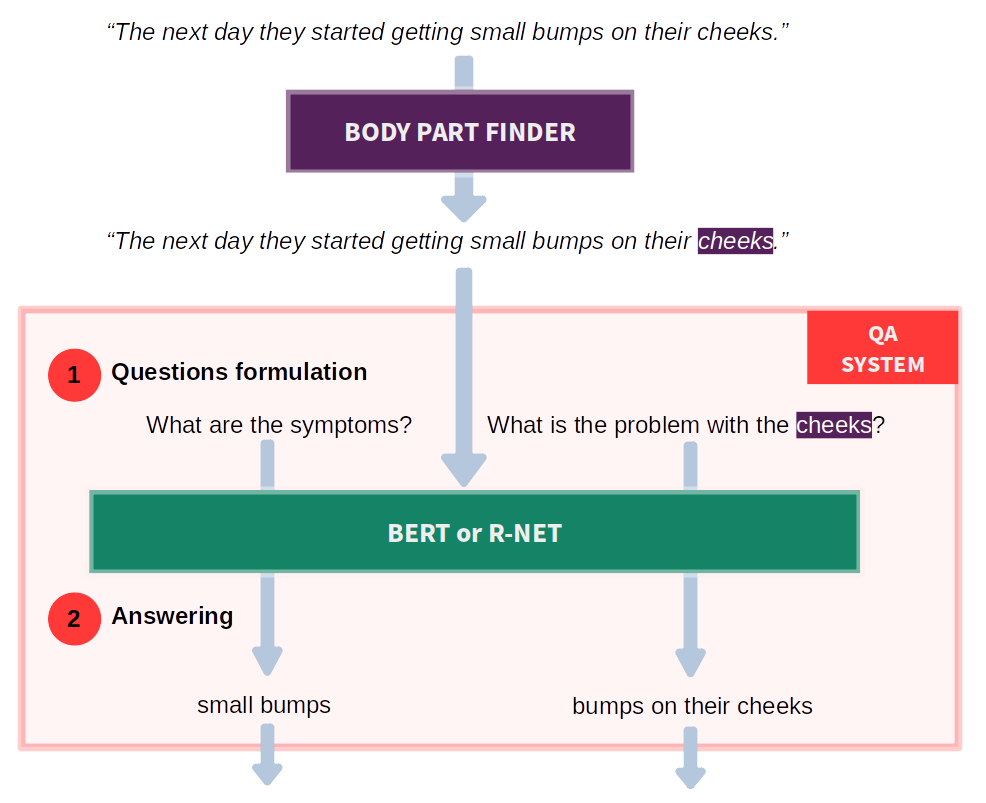
\includegraphics[width=14cm]{qa_sys}
\caption{The \textit{QA system} illustated.}
\medskip
\end{figure}

\subsection{Using BERT for reading comprehension}
\subsubsection{What is BERT?}
\subsection{R-NET}


\section{Answer Interpreter}
\label{sec:answer_interpreter}
TODO


\section{Vectorifier}
\label{sec:body_part_finder}
TODO


\section{Symptom Tree Mapper}
\label{sec:symptom_tree_mapper}
\subsection{Symptom Tree}
TODO, representation in anytree, from mysql following refto

\subsection{Mapping of a token for prediction to a specific symptom}
TODO


\section{How to evaluate results?}
\label{sec:eval_results}
TODO


\section{How to find an internal representation of a symptom?}
Use the concept name and vectorize the sentence (with glove)
Prima fai lo stemming pero', justify it, reduce the space of mapping. possibile figura


\section{Dataset}
site I visited
"extrapolating sentences within the posts" in which there were classifiable symptoms wrt the classification
format of the sentences: xml tags, sentence tag